\begin{figure}
  \setlength{\unitlength}{\textwidth}

        \begin{picture}(1,0.4)(0,0.4)

      % % % Parkinson Data 
%      \put(0.1,1.1){\includegraphics[width=0.75\unitlength]{../FnP/gnuplot/displacement_low_pi_1_plot2.eps}}
%      \put(0.1,0.76){\includegraphics[width=0.75\unitlength]{../FnP/gnuplot/velocity_low_pi_1_plot2.eps}}
      \put(0.1,0.42){\includegraphics[width=0.75\unitlength]{../FnP/gnuplot/mean_power_low_pi_plot2.eps}}
      
%       \put(0.07,0.95){$\displaystyle\frac{V}{D}$}
%       \put(0.07,1.3){$\displaystyle\frac{A}{D}$}
       \put(0.05,0.6){$\displaystyle\frac{P_{m}}{\rho \mathcal{A}U^3 }$}
       \put(0.5,0.4){$\massdamp$}
       \
%\put(0.189,1.415){\small(a)}
%\put(0.189,1.07){\small(b)}
%\put(0.189,0.73){\small(c)}

%  

      
    \end{picture}

  \caption{Dimensionless mean power as a function of \massdamp obtained using QSS assumption at high and low \ \massstiff mean power as a function of \massdamp.. . Data presented at $\massstiff=10 \ (\times)$, \  $\massstiff=0.1 \ $ (\ding{117}), and  \  $\massstiff=0.01 \ \ (\triangle)$.}
    \label{fig:low_pi_1_plot2}
\end{figure}

 %vspace{10cm}
